\section{Introduction to Proofs}

\frame{
{Part 1: Introduction to Proofs.}

\tableofcontents[currentsection,hideallsubsections, firstsection=2, sections={2-5}]
}

\subsection{What is a Proof?}

\begin{frame}{What is a proof?}

  Some concepts are easy to understand, but not easy to show that they are true.\bigskip

  \begin{columns}
    \column{0.3\textwidth}
      \centering
      
\includegraphics[width=.5\textwidth]{../img/triangle_rect}
    \column{0.7\textwidth}
      \begin{itemize}
        \item Pythagoras Theorem:
        \begin{equation*}
          a^2+b^2=c^2
        \end{equation*}
        \item It is easy to show this is true for {\bf any one triangle}.
        \item But how do you show it is is true for {\bf all} triangles?
      \end{itemize}
  \end{columns}
  \bigskip

  The proof of the Pythagoras theorem is {not obvious}: there are more than 100 different proofs!
\end{frame}

\begin{frame}{What is a proof?}{One Pythagoras Proof}

  \begin{columns}[T]
    \column{0.7\textwidth}
      \begin{itemize}
        \item {\bf Proof}: by geometric construction
        \item Arrange four identical triangles;
        \item Show that internal angles are right;
        \item Internal square area: $c^2$
        \item External square area: $(a+b)^2$
        \item $(a+b)^2 = c^2 + 4(\text{area triangle})$
        \item $(a+b)^2 = c^2 + 4(\frac{ab}{2})$
        \item $a^2 + 2ab + b^2 = c^2 + 2ab$
        \item $a^2 + b^2 = c^2$ \hfill $\blacksquare$
      \end{itemize}
    \column{0.3\textwidth}
      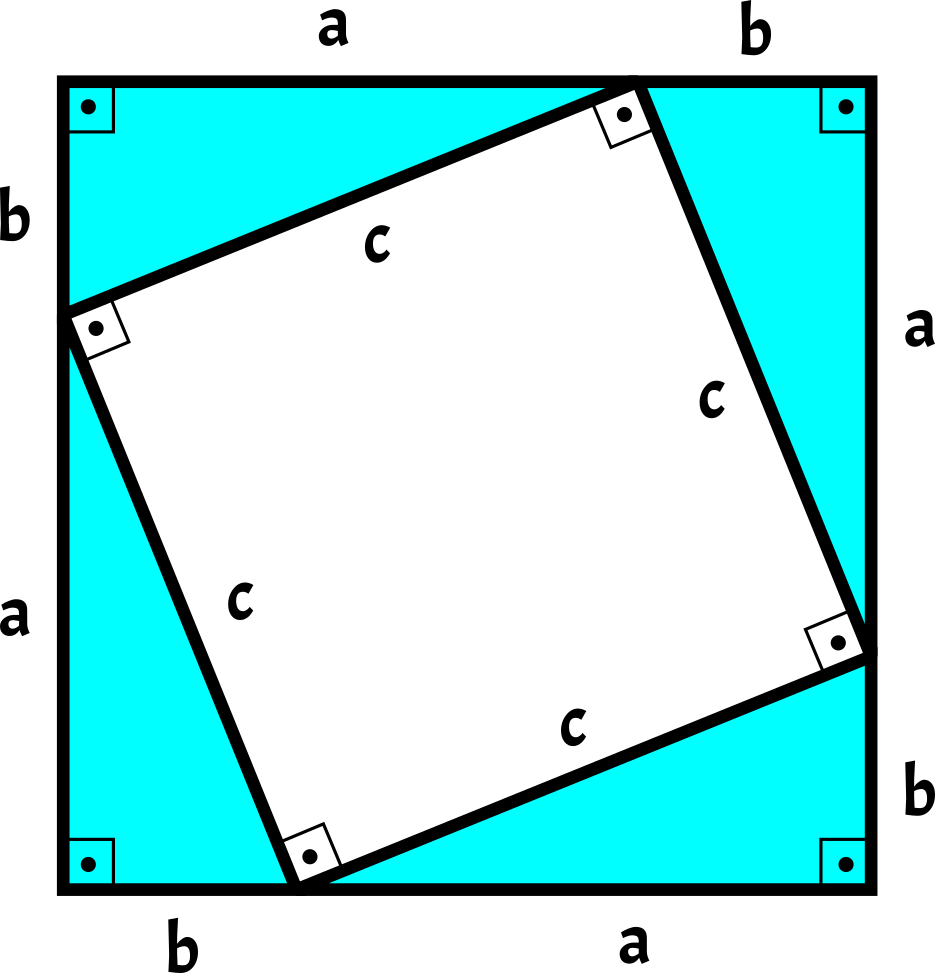
\includegraphics[width=\textwidth]{../img/triangle_pytagoras}
  \end{columns}
  \bigskip

  {\bf Remember:} There are many other possible proofs. (Beautiful proofs, short proofs, wrong proofs, etc.)
\end{frame}

\begin{frame}{False Proofs}{Infinite Chocolate!}
  \begin{center}
    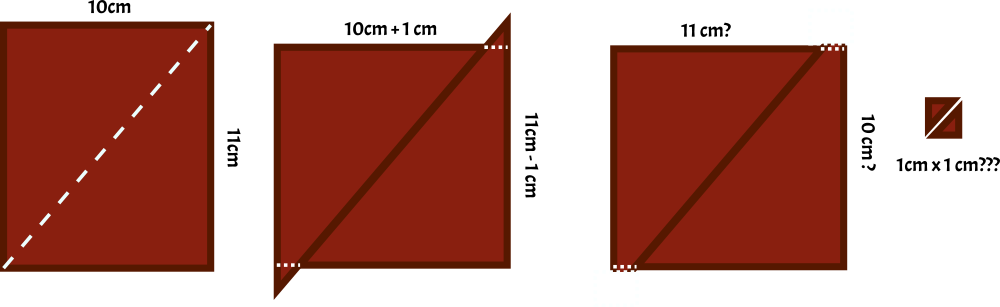
\includegraphics[width=.9\textwidth]{../img/false_proof}
  \end{center}
  \begin{itemize}
    \item What is wrong with the proof above?
    \item \alert{Be careful!} A false proof can have many correct steps, and {\bf only one} impossible step.
  \end{itemize}

  \begin{block}{}
    We can use proofs to show that something is {\bf incorrect} as well!
  \end{block}
\end{frame}

\subsection{Proofs and Computer Science}

\begin{frame}{Proofs and Computer Science}{Why are proofs important for Computer Science?}

  \begin{itemize}
    \item We don't use proofs only for mathematical equations.
    \item We can use proofs to {\bf show that a program is correct}. (or incorrect)
    \vfill

    \item Example cases:
    \begin{itemize}
    \item Use proofs to show that the result of a program is correct for any input;
    \item Use proofs to show that one type of input will cause a bug in the program;
    \item Use proofs to show that a program finishes in $N$ steps;
    \end{itemize}
  \end{itemize}
\end{frame}

\begin{frame}[fragile]{Proofs and Computer Science}{Example:}
  \begin{itemize}
    \item Is the program below correct or incorrect?
    \item Can you show by using a proof?
  \end{itemize}
  \bigskip

\begin{verbatim}
int triangle_type(int a, int b, int c)
  // a, b, c are the length of the sides of a triangle;
  if (a == b)
    if (b == c)
      return "all sides are equal";
    else
      return "two sides are equal";
  else if (b == c)
    return "two sides are equal";
  else
    return "all sides are different";
\end{verbatim}
\end{frame}

\begin{frame}{Next Part:}
  Proof Techniques: How do we prove something?
\end{frame}
